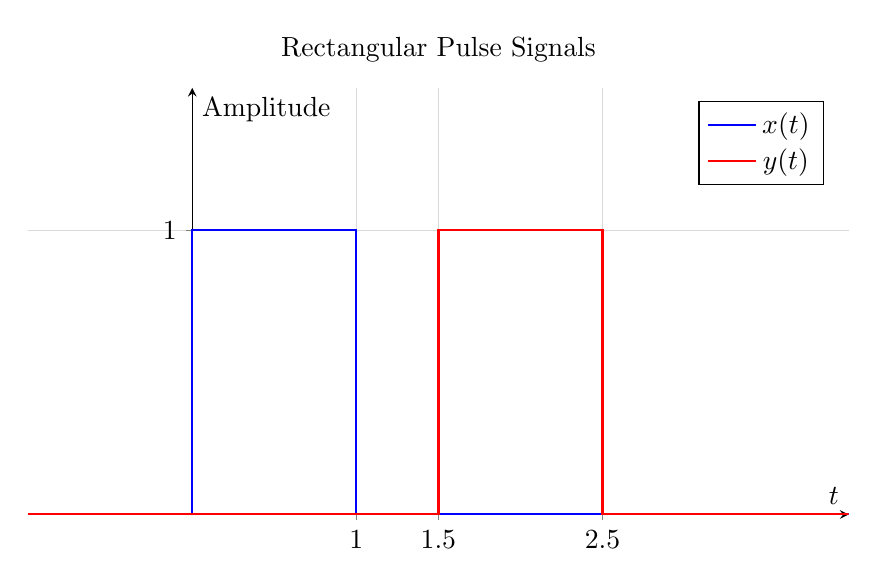
\begin{tikzpicture}
	\begin{axis}[
		width=12cm,
		height=7cm,
		title={Rectangular Pulse Signals},
		xlabel={$t$},
		ylabel={Amplitude},
		axis lines=middle,
		xmin=-1, xmax=4,
		ymin=0, ymax=1.5,
		xtick={0,1,1.5,2.5},
		ytick={1},
		grid=major,
		grid style={line width=.1pt, draw=gray!30},
		legend pos=north east,
		]
		% x(t)
		\addplot+[blue, thick, mark=none] coordinates {
			(-1,0) (0,0) (0,1) (1,1) (1,0) (4,0)
		};
		\addlegendentry{$x(t)$}
		
		% y(t)
		\addplot+[red, thick, mark=none] coordinates {
			(-1,0) (1.5,0) (1.5,1) (2.5,1) (2.5,0) (4,0)
		};
		\addlegendentry{$y(t)$}
	\end{axis}
\end{tikzpicture}